\documentclass{article}
\usepackage[danish]{babel}
\addto{\captionsdanish}{\renewcommand{\abstractname}{Abstract}}

\usepackage[a4paper,top=2cm,bottom=2cm,left=3cm,right=3cm,marginparwidth=1.75cm]{geometry}

\usepackage{amsmath}
\usepackage{graphicx}
\usepackage{subcaption}
\usepackage{minted}
\usepackage[colorlinks=true, allcolors=blue]{hyperref}
\usepackage{url}

\begin{document}

\begin{abstract}
The goal of this project was to explore the feasibility of automating the process of identifying highlights in live-streaming broadcasts using text analysis. This task can be very time-consuming, as it typically requires watching the entire video in order to identify the most notable or interesting moments. By automating this process, the creator of the broadcast can focus on creating content rather than sifting through hours of footage.

To begin the project, research was conducted with the goal of finding the best methods for analyzing chat messages in order to identify highlights. However, difficulties were encountered due to the international user base of the chosen streaming platform, Twitch. By instead focusing on the emotes used, it was possible to make a system that is indifferent to languages.

One of the primary goals of the project was to make the solution as scalable as possible. To achieve this, the system was implemented using a service-oriented system architecture and every implementation detail was carefully researched. Every system component was written using the programming language Rust, which is known for its low resource overhead.

The final system had four primary components: a WebSocket-based chat message collector, a service for analyzing the chat messages, a service for identifying potential highlights, and a service for cutting the original video into highlights. The chat message collector was responsible for gathering all of the messages sent in the chat during the broadcast, the analysis and highlight identification services then used this data to identify patterns or trends that might indicate a highlight. The service then analyzed these patterns and identified the most promising candidates for inclusion in a highlight reel. Finally, the video-cutting service took the identified highlights and created a new video file that included only those segments.

Overall, the system was successful in identifying a number of highlights that would normally require manual review of the entire video. Many of these highlights revolved around the streamer rather than the game itself, which is something that would not be possible using a computer vision-based model. This demonstrates the potential of using text analysis to automate the highlight identification process and allows creators to focus on creating content rather than sifting through hours of footage.
\end{abstract}

\renewcommand{\contentsname}{Indholdsfortegnelse}

\tableofcontents

\section{Indledning}
Inden for live streaming verdenen er en af de primære måder at gro sin audiens gennem deling af højdepunkter på sociale medieplatforme som YouTube, Tiktok og Instagram. Ved deling af højdepunkter får streameren mulighed for at nå ud til en større mængde mennesker, samtidig får fans muligheden for at se højdepunkterne, uden at behøve at se med live.

De tre førnævnte platforme har hvert deres system til at anbefale nye videoer til deres brugere. Disse systemer er bygget til at øge stickinessen på platformen, ved at profilere hvad der er størst sandsynlighed for at brugeren interagerer med \cite{meserole_how_2022}.
Typisk vil det betyder at en person der for eksempel er interesseret i historie, vil blive anbefalet indhold indenfor det emne. Dette øger sandsynligheden for at brugeren kommer tilbage, eftersom brugeren skal bruge mindre tid på at finde indhold de synes er interessant. Dette giver live streaming kanaler en god mulighed for at ramme nye seere indenfor deres primære målgruppe ved at dele mindre segmenter af deres live streams, eftersom de personer som bliver anbefalet indholdet ofte i forvejen er interesseret i spillet.

Indsamlingen af højdepunkter er for de fleste streamere en tidskrævende manuel process, der kræver at streameren ser hele live streamen igennem. Når et højdepunkt bliver fundet skal streameren bruge tid på at redigere i den originale video. Dette er en process som potentielt kan automatiseres ved at analysere live streamen.

Der er som udgangspunkt tré forskellige måder at bygge et system til at analysere livestreams. Første løsning er ved hjælp af computer vision. Analysering ved hjælp af computer vision fungerer ved at lede efter specifikke indikatorer i videoen. I skydespil kommer der for eksempel ofte en indikator når spilleren skyder en modstander. Derved er det muligt at fastlægge hver gang der sker noget interessant i spillet.

Den anden løsning vil være at analysere lyden i hvert segment. Lydgenkendelse fungerer fundamentalt på samme måde som computer vision, den eneste forskel er mediet der bliver analyseret. Ligesom at spil ofte har visuelle indikatorer, har de samtidig audio baserede indikatorer, dette er specielt tydeligt i MOBA spil som League of Legends og DOTA 2, hvor der er specifikke lydeffekt hver gang der sker noget.

Begge løsninger ville kunne bruges til at finde højdepunkter, problematikken med begge ligger dog i at de er yderst statiske. Dette kommer af at både computer vision og lydgenkendelse systemer bliver trænet til at genkende specifikke indikatorer. Systemerne har ikke mulighed for at finde begivenheder som de ikke er blevet trænet til. Dette vil betyde at resultatet af disse løsninger vil være baseret på hvad der sker i spillet under livestreamen. Computer vision kræver derudover en stor mængde data det kan trænes på for at opnå et brugbart resultat, derfor vil det kræve en stor mængde arbejde hver gang et nyt spil skal understøttes.

Den sidste løsnings er at analysere live streaming kanalens chatbeskeder. Ved at analysere chatbeskederne er det potentielt muligt at finde højdepunkter som kræver menneskelig forståelse, hvilket ikke er muligt med de nuværende implementationer af computer vision og lydgenkendelse. Eftersom løsningen vil være bygget op omkring hvordan streamerens primære målgruppe, seerne, reagerede i et givent segment øger det sandsynligheden for at være relevant Dette gør tekstanalyse til en yderst interessant løsning til at automatisere generering af højdepunkter.

Ud fra dette, kan der defineres en problemstilling der fokuserer på at undersøge om det er muligt i praksis:

\textbf{Er det muligt at finde højdepunkter i live streams ved at analysere platformens chat?}

\begin{itemize}
\item Hvordan sikres der at det virker på tværs af flere sprog?
\item Er sentiment analyse et brugbart alternativ til computer vision?
\item Hvilke teknologier er mest optimale?
\item Hvordan sikres der at systemet er skalerbart?
\end{itemize}

\section{Afgrænsning}
Der findes et stort udvalg af forskellige live streaming platformer. Indenfor gaming nichen er Twitch en af de største i den vestlige verden \cite{clement_us_2022}. På baggrund af dette blev der valgt at fokusere på Twitch, målet med systemet er dog på sigt at understøtte flere platforme. Understøttelse af flere platforme burde teoretisk være simpelt når det er blevet bekræftet at systemet virker.



\section{Metodeliste}
\subsection{Brainstorm}
Brainstorming blev brugt til effektivt at danne et overblik over nødvendige system komponenter, samt mulige implementationer \cite{kobenhavns_universitet_klassisk_nodate}
\subsection{Desk research}
Desk research blev brugt til at give en bedre forståelse af hvordan live streaming platforme typisk bliver brugt \cite{albrechtsen_guide_2020}

\subsection{Rapid prototyping}
Under projektet er rapid prototyping blevet brugt til løbende at iterere på system komponenterne \cite{kobenhavns_universitet_hurtige_nodate}.


\subsection{Systemarkitektur diagram}
Der blev løbende udarbejdet diagrammer over systemet med henblik på at finde den bedste mulige implementation \cite{lucidchart_how_2021}

\section{Hvordan analyseres chatten bedst?}

Twitch er en international live streaming hjemmeside, med streamere fra hele verden. Dette betyder at både streamen, samt chatten, kan være i et hav af forskellige sprog. Den brede vifte af forskellige sprog gør det sværere at skalere traditionelle sentiment analyse systemer, eftersom mængden af sprog der skal tages højde for er stor. Med tiden har Twitch dog indirekte fået kreeret deres eget sprog gennem emotes, som er Twitches egen implementation af emojis. Disse emotes har hver deres betydning, hvilket giver seerne mulighed for at udtrykke sig på en måde, hvor andre seere af kanalen øjeblikkeligt kan forstå hvad personen mener, uden de behøver udtrykke det med ord. For eksempel bliver emoten “PogChamp” ofte brugt til at symbolisere at der skete noget spændende \cite{alexander_guide_2018}.

Twitch har en lang række officielle emotes. Når en streamer bliver en del af Twitch partnerskabsprogrammer får de mulighed for at uploade personlige emotes til deres kanal. Dette giver streamerne mulighed for at tilpasse deres kanal, og dermed give seerne en mere personlig oplevelse.

For at bruge en kanals emotes kræver det at seeren har et abonnement. Der findes dog fler tredjeparts browser udvidelser som gør det muligt for streamere, samt seere, at uploade og bruge emotes udenom Twitch officielle system. Disse tredjepart udvidelser bliver samtidig brugt af streamere som streamer på flere forskellige platforme, osse kaldet multistreaming, eftersom det ikke er alle platforme som understøtter emotes.

\subsection{Hastighed på chat}

Når en Twitch kanal får et højt antal seere overgår chatten typisk fra at være en reel samtale mellem streameren og personens seere, til i stedet at være fyldt med emotes \cite{ford_chat_2017}. Dette sker højst sandsynligvis fordi at antallet af beskeder der bliver sendt på store kanaler simpelthen er så højt, at selv hvis streameren prøvede, vil de ikke kunne nå at læse dem alle. Emotes giver dog streameren mulighed for hurtigt at få et indblik i hvad seere tænker, eftersom de som tidligere nævnt har hver deres betydning.

På kanaler med mange seere er en af de potentielt største indikatorer for om hvorvidt der sker noget spændende på live streamen, antallet af beskeder der bliver sendt over en kort tidsperiodet. Ved blot at kigge på antallet af beskeder, udsættes systemet dog for en større risiko af type I (falsk positiv) og type II (falsk negativ) udfald på mindre kanaler.
På mindre kanaler vil der naturligt være chance for store afvigelser i antallet af beskeder, eftersom antallet af unikke personer der bruger chatten i de fleste tilfælde stiger proportionel ud fra antallet af unikke seere.
Disse udfald vil man potentielt kunne mindske ved i stedet for at kigge direkte på antallet af beskeder, kigge på hvilke emotes der bliver brugt. Dette giver mulighed for at vægte emotes der bliver brugt til at indikere noget interessant skete højere end dem som blot bruges under normal samtale.

\section{Design af systemarkitektur}
Inden udviklingen på et nyt system går i gang, er det vigtigt at danne sig et overordnet ide omkring hvad systemet skal kunne. Hertil blev det fastslået at systemet som minimum skulle kunne overvåge en live streaming kanal, samt dens chatbeskeder. Ud fra chatbeskederne skal systemet kunne analyse beskederne, beskederne skal derefter inddeles i mindre tids segmenter med henblik på at finde segmenter der indeholder et potentielt højdepunkt. Til sidst skal højdepunkterne hentes.

\begin{figure}[hp]
\centering
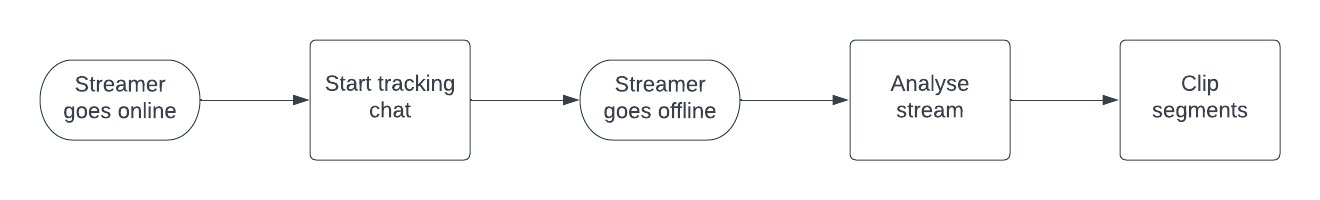
\includegraphics[width=\textwidth]{twitch-highlight-finder-flow.png}
\caption{diagram over flow - eget virke}
\end{figure}

Eftersom at systemet er delt ind i en række forskellige trin, egner det sig godt til en serviceorienteret systemarkitektur. En serviceorienteret arkitektur fungerer ved at dele hvert overordnede funktionalitet ind i dets eget system. Dette er modsætningen til en monolitisk arkitektur hvor der i stedet bliver bygget ét stort system, der indeholder det nødvendige funktionalitet. Fordelen ved en serviceorienteret arkitektur ligger i at det giver mulighed for at skalere hvert enkelt del af systemet uafhængigt af de andre.

Serviceorienteret systemarkitekturer bruger ofte API’er og messaging queues til at kommunikere internt. I dette tilfælde egner en messaging queue sig yderst godt, eftersom de enkelte dele af systemet ikke er direkte afhængig af hinanden. Samtidig kan køen bruges til at distribuere opgaver. Derved kan der skabes et flow mellem systemerne der gør at de enkelte dele af systemet kan være slukket når de ikke har nogen opgaver.

\section{Valg af programmeringssprog}
De største kanaler på Twitch kan sagtens have flere hundredtusind live seere, som sender hundredvis af chatbeskeder i minutter. Derfor er det yderst vigtigt at systemet til at indsamle chatbeskederne er så effektivt som muligt. Med det in mente vil det som udgangspunkt være en fordel at bruge et kompileret sprog, eftersom de gør det muligt at opnå en bedre ydeevne end et fortolket sprog, da de har mindre overhead.

\begin{figure}[hp]
\centering
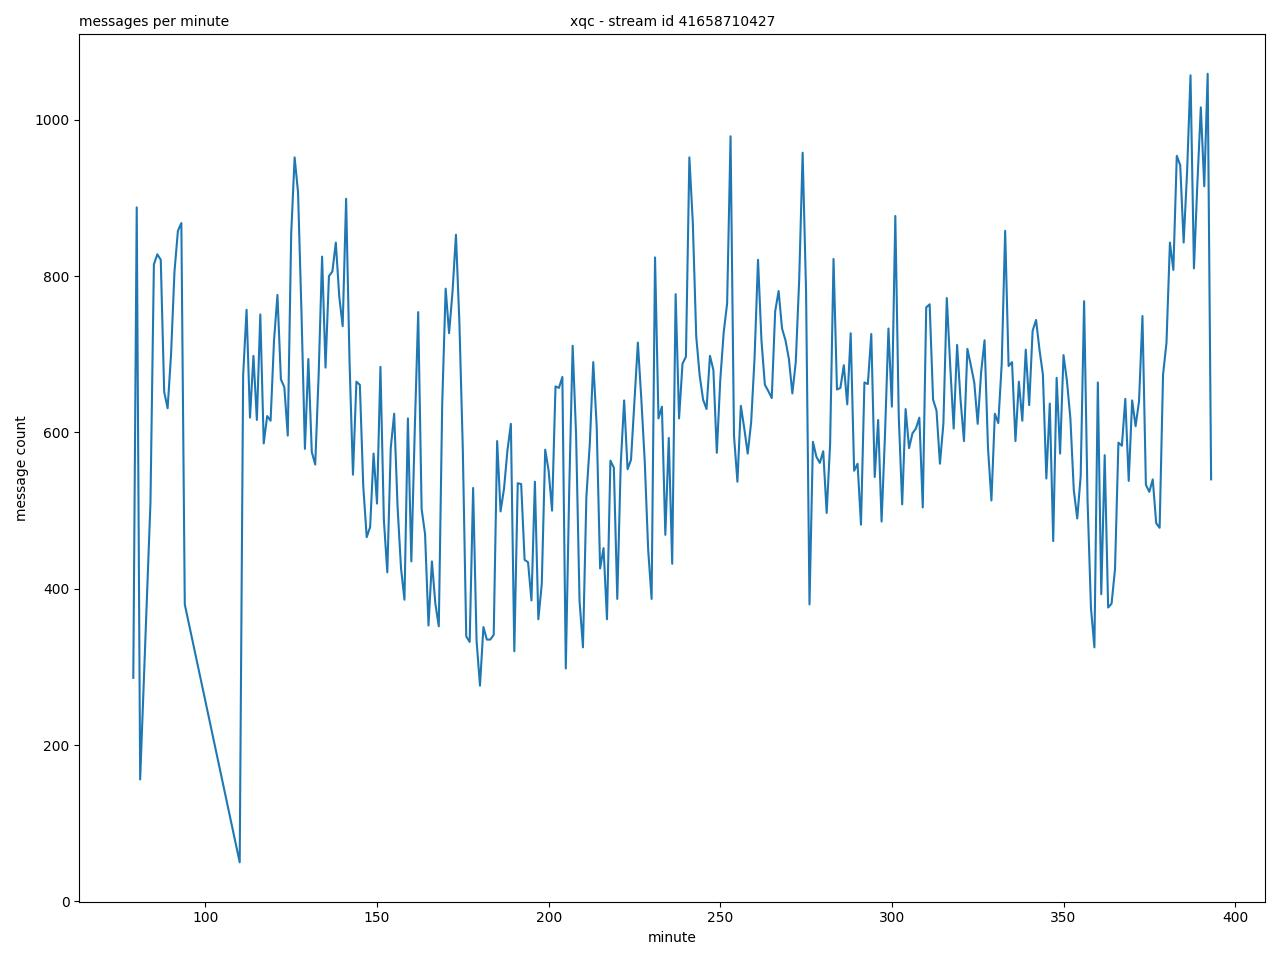
\includegraphics[width=\textwidth]{messages-per-minute-xqc-41658710427.jpg}
\caption{graf over beskeder pr minut - eget virke}
\end{figure}


Når man snakker kompilerede sprog er det umuligt at undgå C og C++. De var begge en mulighed, de blev dog fravalgt på baggrund af at de kræver manuel håndtering af hukommelse, hvilket mindsker udviklingshastigheden samt øge sandsynligheden for fejl \cite{thomas_proactive_2019}. Det betød at valget primært lå imellem Go og Rust, der begge er blandt de mest populære kompilerede sprog med automatisk håndtering af hukommelse.

Begge sprog har deres fordele og ulemper, og der er ikke et decideret bedste sprog blandt de to. Den største forskel, hvis man ser bort fra syntaks, ligger i måden de håndterer hukommelse. Go bruger en mark-sweep tracing garbage collector til at håndtere hukommelse, der fungerer ved løbende at markere alle heap allokeringerne der er refereret til fra call stacken som aktive. Derefter fjernes enhver allokering der ikke er markeret \cite{go_guide_nodate}.

Rust har i modsætning til Go, ikke en indbygget garbage collector. I stedet bruges der en række regler bygget op omkring ejerskab, scope, samt levetid på allokeringer. Disse regler gør det muligt allerede ved kompilering af programmer, at udregne hvornår enhver allokering bør de-allokeres \cite{rust_what_nodate}. Ved at undgå at bruge en garbage collector kan Rust potentielt opnå en bedre ydeevne, fordi der ikke behøves at blive brugt ressourcer på at gennemgå allokeringerne. Garbage collection er en process som i visse tilfælde kan resultere i en øget reaktionstid på et program, da de fleste garbage collectore er nød til kortvarigt at pause programmet \cite{howarth_why_2020}.

Når det er sagt, vil valget mellem Go og Rust realistisk set ikke have en mærkbar forskel for et system af denne størrelse. At Rust bruger mindre hukommelse betyder dog at antallet af kanaler hvert enkelt node kan overvåge er højere, hvilket selvfølgelig er en fordel.


\section{Data storage}
Til data storage blev MongoDB valgt, da det gør det muligt at iterativt ændre database designet uden behov for at migrere eksisterende data.
MongoDB understøtter også tidsbaserede kollektioner, men denne funktion blev ikke benyttet i dette projekt, da den har en række begrænsninger, der gør det svært at ændre på dokumenterne efter de er indsat \cite{mongodb_time_nodate}. Det ville ikke desto mindre være en mulig optimering.

En traditionel SQL database som PostgreSQL ville sagtens kunne være brugt i stedet, det ville dog have den indvirkning at der skulle bruges mere tid til at planlægge database designet på forhånd.

\section{Indsamling af chatbeskeder}
Twitch tilbyder mulighed for at forbinde til deres Internet Relay Chat Protocol (IRC) server, der er et tekstbaseret chat system med formålet at kunne sende beskeder til flere enheder på samme tid. Alle klienter forbinder til en server, hvorefter de kan sende og lytte til beskeder fra hinanden. Dette gør IRC til en effektiv måde at opbygge et chat system til en live streaming platform som Twitch. IRC har en standardiseret implementation, hvilket gør det nemt at udvikle nye klienter \cite{oikarinen_internet_1993}.


Twitch tilbyder to forskellige måder at lytte på deres IRC server, enten gennem traditionelle IRC klienter eller WebSockets \cite{twitch_twitch_2022}.

WebSockets er en netværksprotokol der gør det muligt at sende data to vejs mellem klient og server \cite{melnikov_websocket_2011}. Dette er en kæmpe fordel når der er tale om systemer der skal kommunikere i realtid, eftersom serveren har mulighed for at sende data til klienten, uden at klienten behøver at anmode om det. Det betyder samtidig at der ikke behøves bruge tid og ressourcer på at oprette en ny forbindelse hver gang at klienten vil anmode om data, da forbindelsen først bliver lukket når klienten, eller serveren, beder om det.

Eftersom at begge løsninger i sidste ender bruger IRC, gør det fra et teknisk perspektiv ikke stor forskel hvilken løsning. WebSockets kan dog have en smule mere forsinkelse, eftersom Twitch intern konvertere det til en IRC besked.

Den største faktor i valget mellem de to ligger i udbredelsen af protokollerne. WebSockets er understøtte af de fleste moderne browsere \cite{caniuse_websockets}, hvilket har resulteret i at protokollen bliver brugt til mange systemer der kræver to vejs kommunikation mellem klient og server \cite{murley_websocket_2021}. IRC derimod bliver kun brugt til chat servere, dette giver WebSockets en klar fordel eftersom det er nemmere at finde dokumentation.
Denne forskel i brug er tydelig når der sammenlignes mellem antallet af downloads af irc \cite{cratesio_irc_nodate}, det mest populære irc bibliotek til Rust, og Tungstenite \cite{cratesio_tungstenite_nodate}, det mest populære WebSocket bibliotek. Tungstenite har på nuværende tidspunkt over 150 gange så mange downloads som irc. Tungstenite indeholder dog både en klient, og server implementation, hvilket påvirker antallet af downloads.


\subsection{Gemning af chatbeskeder}
Implementationen af besked indsamleren bestod af en tråd, der var dedikeret til at lytte efter nye beskeder. Når en ny besked blev fundet, blev den sendt gennem en kanal til en anden tråd, der håndterede beskeden. Denne løsning blev valgt for at minimere latenstiden mellem at en besked bliver fundet, til den er færdig analyseret.

Til at starte med blev beskederne grupperet, hvorefter de løbende blev gemt i en kollektion. Dette virkede upåklageligt lige indtil der blev tilføjet store live streaming kanaler. Denne stigning af beskeder synliggjorde et stort problem med den originale implementation. På grund af at analyse systemet blev nød til at tjekke hele kollektionen for nye beskeder, steg antallet af database operationer markant. Det kombineret med at antallet af operationer i værste tilfælde lå på 3 per besked \((insertMany -> find -> updateOne)\) , og i bedste tilfælde \((1 + 1 + n)\) operationer per gruppe af beskeder, betød at den daværende løsning potentielt ville have svært ved at skalere.

Ved at lægge en messaging queue imellem indsamleren og analysatoren blev antallet af operationer per besked reduceres til maksimalt 1. Det reducerede samtidig tiden der gik fra en besked blev indsamlet, til at den var færdig analyseret, eftersom køen gjorde det nemmere at distribuere analysing ud på flere maskiner.

\subsubsection{Valg af message queue}
Der er et stort udvalg af forskellige kø systemer på markedet, heriblandt RabbitMQ, ZeroMQ og Kafka. Disse systemer har hver deres fordele og ulemper. I dette projekt var der ikke nogen specifikke tekniske behov til kø systemet, dette gjorde det muligt at vælge kø ud fra andre parameter.

AWS SQS (Simple Queue Service) blev valgt, fordi det har en prismodel som er bygget op omkring pay-per-use, dette betyder at i stedet for at betale en fast pris om måneden, betales der kun for de ressourcer der bliver brugt. Denne prismodel er utrolig brugbar i udviklingsfasen af et projekt, eftersom det gør det nemt at teste implementationen af et system uden at betale for idle usage. Samtidig skalerer systemet automatisk ud fra brug, hvilket er en kæmpe fordel, specielt fordi antallet af beskeder varierer drastisk ud fra hvilke kanaler der er online.
Alt i alt var valget af AWS SQS som kø system det rette valg for dette projekt, grundet de mange fordele og den fleksible prismodel.

\subsubsection{Valg af SQS kø type}
SQS tilbyder to forskellige typer køer, Standard og FiFo (First-in, First-out).

En FiFo kø fungerer på samme måde som en kø i et supermarked fungerer, den forreste person (besked i dette tilfælde), bliver håndteret først. Denne type kø er brugbart når rækkefølge af beskederne er kritisk. SQS FiFo implementationen garanterer samtidig at en besked kun bliver leveret til en consumer en gang \cite{amazon_sqs_queue_types}.

SQS Standard køen giver hverken en garanti for rækkefølgen af beskeder, eller at en besked ikke bliver leveret mere end en gang. I stedet ligger fokus på standard kø typen på at kunne levere så mange beskeder som muligt. Dette sker ved at distribuerer beskederne ud på flere servere af gange med det formål at forbedre tilgængeligheden og skabe redundans \cite{amazon-standard-queue}.

Chat beskederne har i forvejen en firevejs sammensat unikt index i MongoDB kollektionen (afsender, kanal, besked, tidspunkt), hvilket garanterer at den samme chatbesked ikke kan blive gemt flere gange. Derfor har hverken rækkefølgen af beskederne, eller duplikere beskeder nogen indvirkning på systemet. Den øgede throughput er dog en kæmpe fordel, eftersom at det gør det muligt at skalere et til højere antal kanaler.

\section{Hentning af emotes}
Til at starte med blev der antaget at det primært var officielle Twitch emotes der blev brugt. Derfor blev der bygget et system til at hente emotes fra alle kanalerne der blev tracket. Hvert enkelt emote blev derefter annoteret på en skala fra et til ti, ud fra om hvorvidt de bliver brugt når der sker noget interessant.

For nemt at kunne annotere emotene blev der bygget en intern frontend til denne del af systemet. Eftersom at frontenden kun er tiltænkt internt brug blev der ikke lagt vægt på hverken design eller user experience. Hvis det havde målrettet brugere ville det selvfølgelig have været en vigtig del at tage højde for.
Frontenden blev bygget i frameworket Next. Next er et React baseret framework der gør det muligt at lave server side renderede applikationer. Dette valg blev truffet fordi at Next gør det muligt at lave server side api ruter, hvilket betød at der ikke var behov for at lave en selvstændig API, blot til frontenden.

TypeScript, som er et syntaktisk supersæt af JavaScript der tillader annotering af datatyper, blev brugt for at sikre at enhver operation stemmer overens med det forventede. I projekter der bruger TypeScript er det nemmere at finde datatype relaterede fejl, eftersom transpileren som udgangspunkt ikke vil oversætte kode fra TypeScript til JavaScript den mener er forkert. Det er dog stadig muligt at lave datatype relaterede fejl, eftersom at TypeScript kun validerer ved transpilering, og ikke under runtime.

Under nærmere analyse af chatbeskederne blev der dog hurtigt tegnet et billede af at denne antagelse var yderst forkert. Grafen nedenunder viser hvilket emotes der er forekommet mest under en live stream på kanalen XQC. Af de hundrede tusinde emote der er blevet brugt under streamen er over 50\% fra tredjeparts udvidelser. Derfor blev det en nødvendighed at indsamle emotene fra de to største tredjeparts udvidelser, BetterTTV og FrankerFaceZ.

\begin{figure}[hp]
\centering
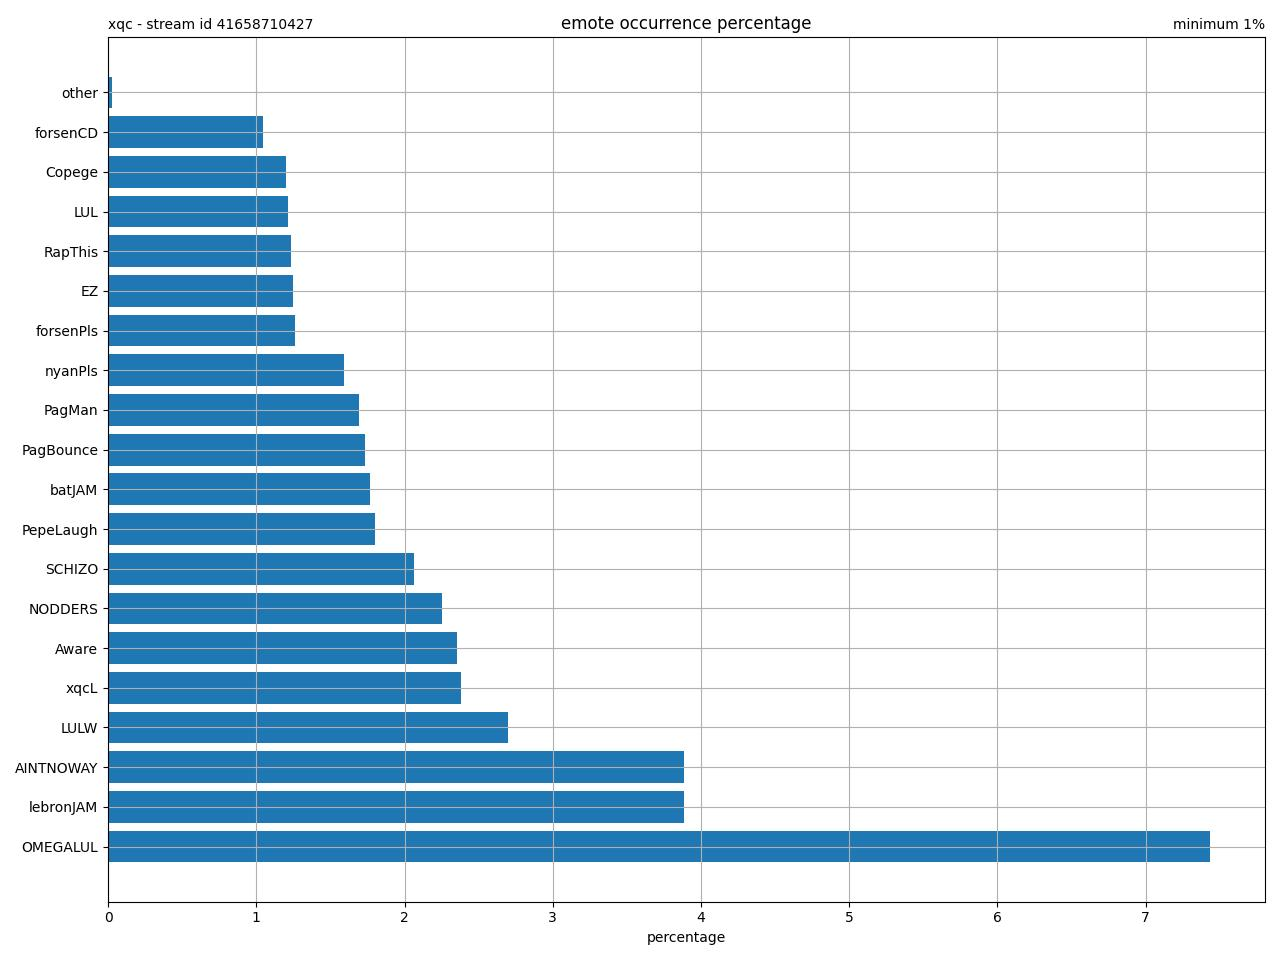
\includegraphics[width=\textwidth]{emote-occurence-xqc-41658710427.jpg}
\caption{mest hyppigt forekommende emotes på xqc stream - eget virke}
\end{figure}

Disse tré data indsamlere blev bygget til at kunne køres som cronjobs. Denne implementations detalje blev valgt fordi at tredjeparts udvidelserne tillader seere at uploade emotes, hvilket øger frekvensen i hvor ofte der bliver lavet nye drastisk.

At inkludere tredjeparts emotene havde den effekt at antallet af emotes gik fra at være et par hundrede, til tyve tusind. Dette betød at var umuligt at annotere størstedelen af de nye emotes. Derfor blev kun de mest populære annoteret. Det betyder at størstedelen af tredjeparts emotene bliver vægtet lavere end tilsvarende officielle, hvilket kan have haft en betydning for de klips systemet har genereret.

I et ideelt system ville værdien af hver emote blive fundet ved først at finde højdepunkter i en stor mængde livestreams, og derefter kigge på hvor ofte en given emote forekommer. Ud fra dette data vil det være muligt at træne en natural language processing (NLP) model der mere præcist kan forudsige værdi af den enkelte emote.

\section{Klipning af højdepunkter}
For at kunne attribuere beskederne fra live stream til en video, var det en nødvendighed at bygge et system til at holde styr på hvornår en live stream var ovre. Her tilbyder Twitch et REST api endpoint der gør det muligt at se hvilke videoer der ligger tilgængelig på en kanal. Når en live stream er færdig bliver live streamen automatisk lavet om til en video, information omkring live streamen og videoen bliver derefter tilgængelig gennem endpointet. Denne data bliver indsamlet løbende gennem et cronjob, for at sikre at enhver ny video automatisk bliver gemt.

Når en ny video bliver fundet sendes det videre til et sekundært system der står for at finde tidspunkter i live streamen hvor der potentielt er et højdepunkt. Dette fungerer ved at segmentere beskederne i buckets af 10 sekunder ud fra hvornår de blev sendt. Derefter får hvert segment en overordnet værdi ud fra summen af de individuelle beskeder. De segmenter med højest værdi bliver sendt videre til systemet der står for at klippe videoen. Hvis der er segmenter der tidsmæssigt ligger tæt bliver de slået sammen, for at sikre at længere højdepunkter ikke bliver skåret op i flere klips.
Til sidst henter systemet til at generere højdepunkterne videoen, og klipper de segmenter der menes at indeholde ud. Højdepunkterne bliver efterfølgende gemt i en AWS S3, hvilket er en cloud-lagringstjeneste til gemning af statiske filer.

\section{Endelig løsnings}
Den endelige systemarkitektur minder konceptuelt om en udvidet ETL data pipeline. En ETL pipeline er en måde at opdele data indsamling i tre faser \cite{fatima_2022}. Første fase, kaldet extract \((E)\), omhandler udtrækningen af data fra en datakilde, i dette tilfælde Twitchs WebSocket. Derefter bliver det sendt videre til transformationsfasen \((T)\) hvor dataen først bliver renset for irrelevante dele, derefter bliver det transformeret til det nødvendige schema \((analyse delene)\). Til sidst bliver dataen loadet \((L)\) ind i en data storage løsning af klipperen.

Alle dele af systemet, undtagen besked indsamleren, blev bygget med henblik på at kunne køre som serverless funktioner ved hjælp af AWS Lambda. Lambda er AWS’ implementation af serverless computing. Serverless computing gør det muligt at køre programmer på en as-needed basis, hvilket vil sige at i stedet for at have en række dedikerede nodes til at køre hvert service konstant, startes hver del i stedet op når der er brug for det. Når programmet har løst sin opgave lukkes det automatisk igen. Derved bliver der kun brugt ressourcer når det er relevant \cite{cloudflare_what_nodate}.

Dette viste sig dog at være mere tidskrævende end forventet, eftersom at Lambdas container runtime på nuværende tidspunkt kun understøtter containere der kan køres på musl baseret Linux distributioner \cite{amazon_using_sdk}. Rust kompileren bruger nemlig som standard glibc til dynamisk linkning på Linux \((x86_64-unknown-linux-gnu)\), hvilket betyder at størstedelen af alle biblioteker er bygget ud fra det faktum. Det betyder samtidig at alle eksterne biblioteker der er kompileret med glibc skal kompileres på ny. Heldigvis var det et problem der var forholdsvist ligetil at løse efter at fejlen blev fundet.

Valget om at bruge AWS som cloud provider blev truffet baseret på at der i forvejen blev brugt AWS SQS som kø system. Et tilsvarende system ville kunne blive bygget med Azure som cloud provider ved i stedet at bruge for at bruge Azure Queue Storage som messaging queue, Azure Blob til at gemme video filerne og Azure Functions \((eller Azure Container Apps)\) til serverless computing.

Det samme ville kunne opsættes i Google Cloud, der ville Google Cloud Tasks kunne bruges til at distribuere opgaver, Google Cloud Storage til filer og Google Cloud Run \((eller Google Cloud Functions\)) som serverless FaaS.
\begin{figure}[!ht]
\centering
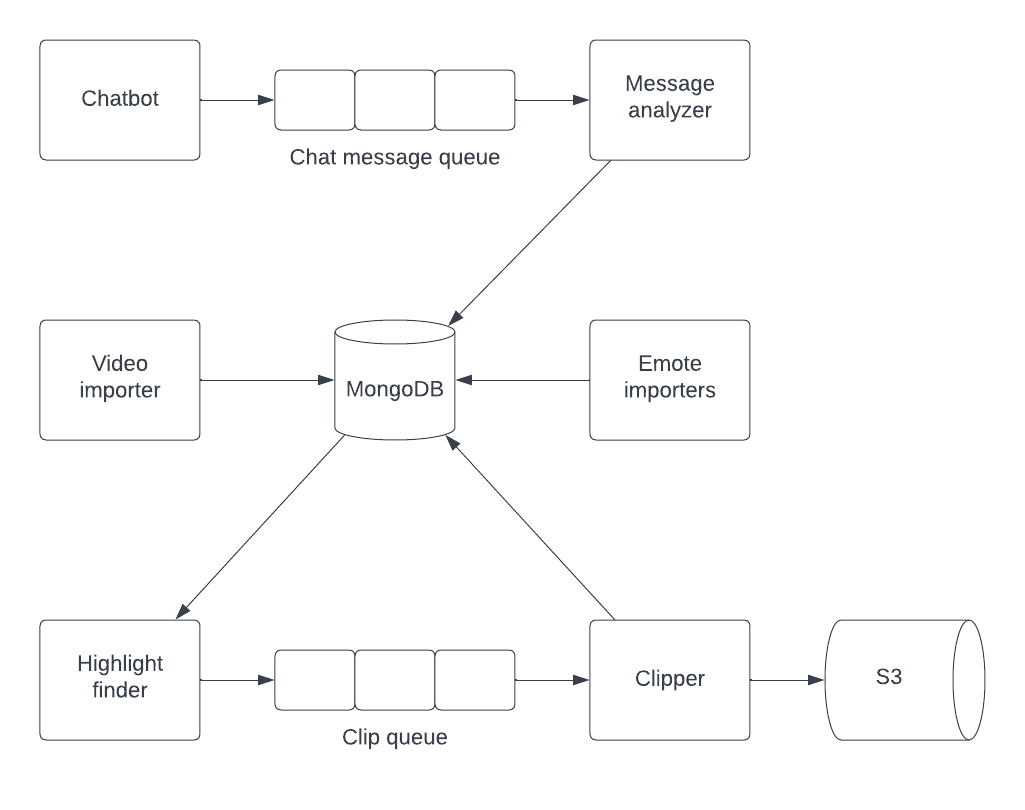
\includegraphics[width=\textwidth]{highlight-finder-overall-diagram.png}
\caption{endelige flow mellem systemet - eget virke}
\end{figure}


\section{Diskussion}


\subsection{Vurdering af chatbeskeder}
Under dette projekt har fokus ligget på at undersøge hvorvidt det er muligt at finde højdepunkter i live streams. Men eftersom det primære fokus i sidste ende lå på backend implementationen mellem de forskellige komponenter, og ikke selve tekstanalysen, er der indirekte blevet lavet en række mindre uforudsete begrænsninger. Den begrænsning der realistisk set har haft størst betydning for det endelige produkt, var at ikke træne en dedikeret natural language processing model (NLP) til at analyse beskederne, i stedet blev højdepunkterne fundet ved at kigge på segmenter af videoen hvor der var højere besked værdi, gennem ren matematik. Set i bakspejlet er det en begrænsning som ikke burde være lavet, eftersom at det resultere i at systemet analyse ydeevne er lavere end det kunne have været. Med en NLP model ville det have været muligt at inkrementalt forbedre analyse evnen, ved at annotere i forvejen kendte højdepunkter, på den måde ville der sikres at systemet ikke har et menneskeligt bias, men i stedet kigger på rådata.

\subsection{Tekst analyse kontra computer vision  }
Tekst analyse og computer vision bør i dette tilfælde ikke ses som direkte konkurrenter, eftersom de har to meget forskellige måder at løse problemstillingen på. Hvor computer vision ofte leder efter specifikke objekter eller tekst i et billede/video gennem objekt detektion og/eller OCR, er tekstanalyse en del mere “fuzzy”. Eftersom sprog kan være meget tvetydige, og ofte kræver kontekst for at forstås kræver det en mere åben tilgang. Dette betyder at et computer vision baseret system vil kunne være mere præcist end tekst analyse. Et tekstanalyse baseret system vil dog kunne finde højdepunkter som er umulig at finde gennem computer vision, eftersom de kræver en “menneskelig” forståelse.

Den største fordel ved at bruge tekstanalyse frem for computer vision ligger dog i mængde af ressourcer det kræver. Computer vision er ofte så ressourcekrævende at den bedste løsning er at køre det på dedikerede grafikkort, derfor kan det være utrolig dyrt at skalere (Fung u. å.). Simpel tekst analyse er dog generelt en del simplere rent beregningsmæssigt, eftersom det ikke er nødvendigt at bearbejde store mediefiler. Når det er sagt er det yderst afhængig af hvilken arkitektur modellen er baseret på, samt formålet med modellen, for eksempel findes der en lang række computer vision modeller der er målrettet IoT og embeddede enheder. Disse modeller er per automatik nød til at bruge en lav mængde ressourcer på grund af begrænsningerne (Roth et al. 2022). Avancerede modeller vil altid være mere krævende, uafhængigt af modeltype. OpenAIs GPT-3.5 baserede chatbot ChatGPT er anslået til kræve som minimum fem Nvidia A100 GPUer blot for at loade modellen (Goldstein 2022).

Den bedste løsning ville være at lave en kombination af begge systemer. Dette vil gøre det muligt at få den bredeste type af højdepunkter, samtidig ville højdepunkterne der bliver fundet gennem computer vision kunne bruges til at forbedre chat analysen.

\subsubsection{Analyse af lyd }
Analysering af lyd er som tidligere nævnt en mulig måde at automatise højdepunkt genererings processen. Dette er dog den løsning som i realiteten er sværest at implementere. Ved computer vision bliver hvert frame der skal processeres typisk konverteret til matricer der afspejler billedet, dette gøres med formålet at lave operationerne nemmere. Lyd er dog fundamentalt bygget op af en række bælgefrekvenser med forskellig intensitet, hvilket betyder at det er en del mere komplekst at transformere om til en let bearbejdeligt datastruktur. Det betyder at det svære at arbejde med for både udvikler og computer. Ud over det findes de fleste indikatorer i spil i forvejen i visuel form, derfor er det heller ikke en løsning der i denne kontekst vil skabe en unik værdi.


\section{Kommerciel værdi }
Ved tekstanalyse har mængden af data der kan analyseres en stor indvirkning på det endelige resultat. Dette betyder at tekstanalyse primært er brugbart på store kanaler, hvor der er tusindvis af seere. På kanaler med få seere vil sandsynligheden for at få et type I \((falsk positiv)\) og type II fejl \((falsk negativ)\) være markant højere.

Ved primært kun at kunne få positive resultater på store kanaler fjernes størstedelen af den primære målgruppe som indtægtskilde. Derfor er den kommercielle værdi af tekstanalyse lavere end computer vision. Computer vision er indifferent over for hvor mange seere der er, det eneste der tages højde for er de specifikke indikatorer som modellen er blevet trænet til at finde.

Automatisk generering af højdepunkter har dog en potentiel kommerciel værdi. Dette kan blandt andet ses ved at kigge på virksomheden Athenascope, som i 2019 rejste en investeringsrunde på \$2.5 millioner \cite{crunchbase_athenascope_nodate}.

\section{Konklusion}
Ved hjælp af systemet blev der genereret 50 forskellige højdepunkter. Størstedelen af disse højdepunkter omhandler streameren der reagere højlydt til hvad der sker i spille.
Af de 50 clips var 11 af dem hvad man indenfor spil verdenen ville kalde et “traditionelt” højdepunkt, hvor spillerne ved hjælp af deres evner vinder over modstanderen.

Overordnet anses dette resultatet for at være en success eftersom det bekræfter at det er muligt at automatisere processen til at finde højdepunkter. Det viser samtidig at chatbeskeder kan være en indikator for hvornår der sker noget interessant.

Sammenlignet med computer vision, giver tekstanalyse mulighed for at finde en type højdepunkter som ikke er direkte relateret til et specifik indikatorer. Disse højdepunkter er ofte fokuseret på den menneskelige aspekt af streameren, i stedet for den mekaniske i spillet. Dette er vigtigt at have in mente for streameren, eftersom at de to forskellige typer af videoer ikke nødvendigvis vil blive set af de samme målgruppe. Højdepunkter hvor det primære fokus ligger på spillet vil ofte ramme en bredere målgruppe, hvorimod at højdepunkter hvor streameren er i fokus er bedre til at skabe en fanbase.

Der bør dog laves en række finpudsninger for at minimere sandsynligheden for at få dårlige udfald. Det der vil have størst indflydelse på kvaliteten af højdepunkterne ville være at skifte til en datadreven model til at vurdere emotes. Den nuværende manuelle process er ikke skalerbar, eftersom det kræver en dyb forståelse af hvordan seerne bruger de forskellige emotes. Den bedste løsning ville være at bygge en natural language processing model ved at annotere en stor mængde live streams for højdepunkter. Derefter bør der beregnes hvor ofte de forskellige emotes fremgår. Det vil samtidig give mulighed for at annotere hver emote ud fra hvilken kontekst den bliver brugt.

Ved at bygge systemet op omkring en servicearkitektur blev skaleringen af de forskellige dele yderst nem. Dette blev specielt tydeliggjort efter at der blev implementeret en messaging queue til chatbeskeder, da det blev muligt at distribuere ud over et højere antal nodes.

Valget på Rust som programmeringssprog betød at ikke var nogen dele af systemet der havde ressource relaterede bottlenecks. Dette var specielt tydeligt under livestream fra streameren XQC, hvor antallet af beskeder i minuttet i visse tilfælde overskrider tusind.

\bibliographystyle{apalike}

\bibliography{sample}

\section{Bilag}

\subsection{Bilag 1 - Repository}
Projektet kan findes på \url{https://github.com/hougesen/twitch-highlight-finder/}

\subsection{Bilag 2 - video filer}
En række generede klips kan findes i "generated-highlights" mappen. Alternativt ligger filerne osse tilgængelig i repositoriet, \url{https://github.com/hougesen/twitch-highlight-finder/generated-highlights}

\end{document}
